\chapter{Optimizing SteelEagle Performance}

As explained in \cref{sec:overview}, the performance of the SteelEagle system
determines its versatility. A drone that is slow to react will be unable to
effectively navigate obstacle-dense environments. The chances of the drone
losing track of a fast on-ground target that is moving erratically increases
substantially if the drone is slow in keeping the target centered in its view.
Given the importance of performance, this chapter details how performance is
defined for SteelEagle, how it is measured, and work done to identify
performance bottlenecks and optimize the system.

\cref{sec:exp1} describes initial efforts to optimize the system that yielded a
more than two-fold reduction in drone-to-cloudlet latency, discovering negative
scale-out attributes of FFmpeg, a video decoding library.  \cref{sec:exp2}
describes subsequent efforts to establish a more systematic approach to
profiling SteelEagle, which found the encoding of the RTSP video stream
generated by the drone to be the biggest contributor to latency.

\begin{figure}[htbp]
\centerline{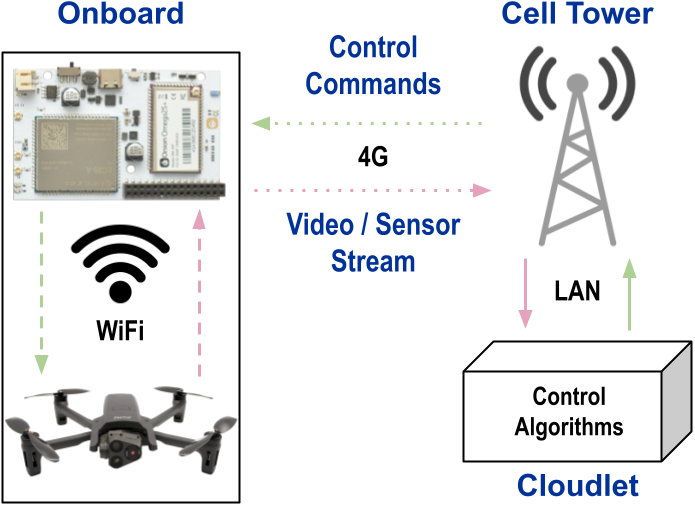
\includegraphics[width = .5\textwidth]{figs/fig-simplified-arch.png}}
\caption{SteelEagle Edge Offload Pipeline}
\label{fig:simplified-arch}
\end{figure}

\section{How is performance defined in SteelEagle?}
\label{sec:steeleagle-performance-def}

The performance of SteelEagle is determined by the end-to-end latency and
throughput of the system. \cref{sec:overview} explained how drones in
SteelEagle are treated as thin clients, with the use of a communications relay
to make up for the lack of cellular connectivity on commerical-off-the-shelf
(COTS) drones. The sensor stream from the drone is forwarded to the
communications relay over Wi-Fi, which in turn forwards it to the cloudlet over
4G LTE. After performing inference on the received data, the cloudlet sends
back piloting commands to the drone, via a hop through the communications relay
(\cref{fig:simplified-arch}). As a result, the end-to-end performance is
determined by several components of the pipeline:
\begin{enumerate}
    \item[(a)] On-drone sensing
    \item[(b)] On-drone pre-processing
    \item[(c)] Tranmission to cloudlet
    \item[(d)] Cloudlet processing
    \item[(e)] Transmission to drone
    \item[(f)] Drone post-processing
    \item[(g)] Drone actuation
\end{enumerate}

Each of these components has a latency associated with it, and a throughput
that it is capable of. The performance of components (a), (b), (f), and (g) is
fixed for a given drone. Factors such as the drone camera's sensor readout time
and shutter speed used affect the frame capture latency, and thus determine the
performance of component (a). Component (b) consists of any processing of the
sensor data before it is transmitted from the drone. The generation of an H.264
stream, for instance, adds latency since the compression process is
computationally intensive, involving analysis of deltas between successive
frames.

For components (c) and (e), performance is determined by the cellular network
used for communication between the relay and the cloudlet. While there is
variance associated with the performance of these components, factors such as
the number of network hops, distance between the relay to the cloudlet, and the
network signal strength available to the relay largely determine the 99th
percentile value of their latency and throughput over a longer period of time.
The performance of component (d) can vary largely based on whether decoding of
the drone stream data is required and type of inferencing that is performed. A
DNN with a complex architecture, for instance, can take much longer for
inference than a traditional computer vision approach. The same inference can
also take less time on a more powerful cloudlet.

\begin{figure}[htbp]
\definecolor{observe-color}{RGB}{175,208,149}
\definecolor{orient-color}{RGB}{255, 255, 166}
\definecolor{decide-color}{RGB}{255,170,149}
\definecolor{act-color}{RGB}{224,194,205}
\centering
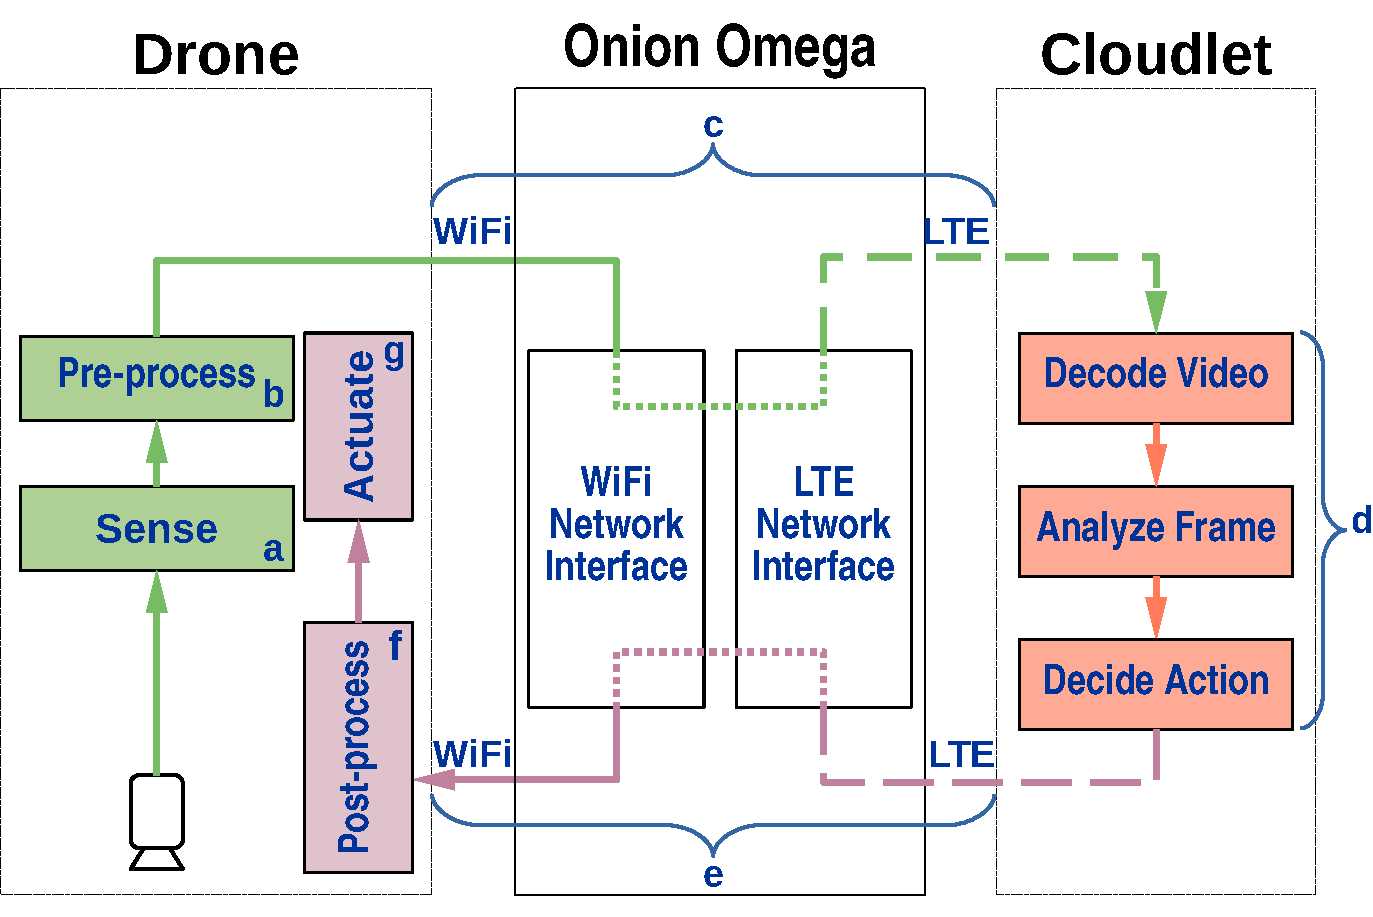
\includegraphics[width = .6\textwidth]{figs/fig-ooda-loop.pdf}\\
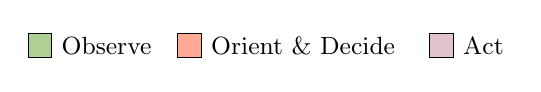
\begin{tikzpicture}
    \draw[fill=observe-color] (1.0,0) rectangle (1.3,0.3);
    \node[right] at (1.3,0.15) {\small Observe};

    \draw[fill=decide-color] (2.9,0) rectangle (3.2,0.3);
    \node[right] at (3.2,0.15) {\small Orient \& Decide};

    \draw[fill=act-color] (6.1,0) rectangle (6.4,0.3);
    \node[right] at (6.4,0.15) {\small Act};
\end{tikzpicture}
\caption{Mapping the SteelEagle pipeline to the OODA loop}
\label{fig:ooda-mapping}
\end{figure}

\Cref{fig:ooda-mapping} shows how these components can be mapped to the various
stage of the OODA pipeline. The ``Observe'' phase includes components (a), (b),
and (c). Components (d) maps to the ``Orient'' and ``Decide'' phases. Finally,
components (e), (f), and (g) correspond to the ``Act'' phase.

\begin{figure}[htbp]
\centerline{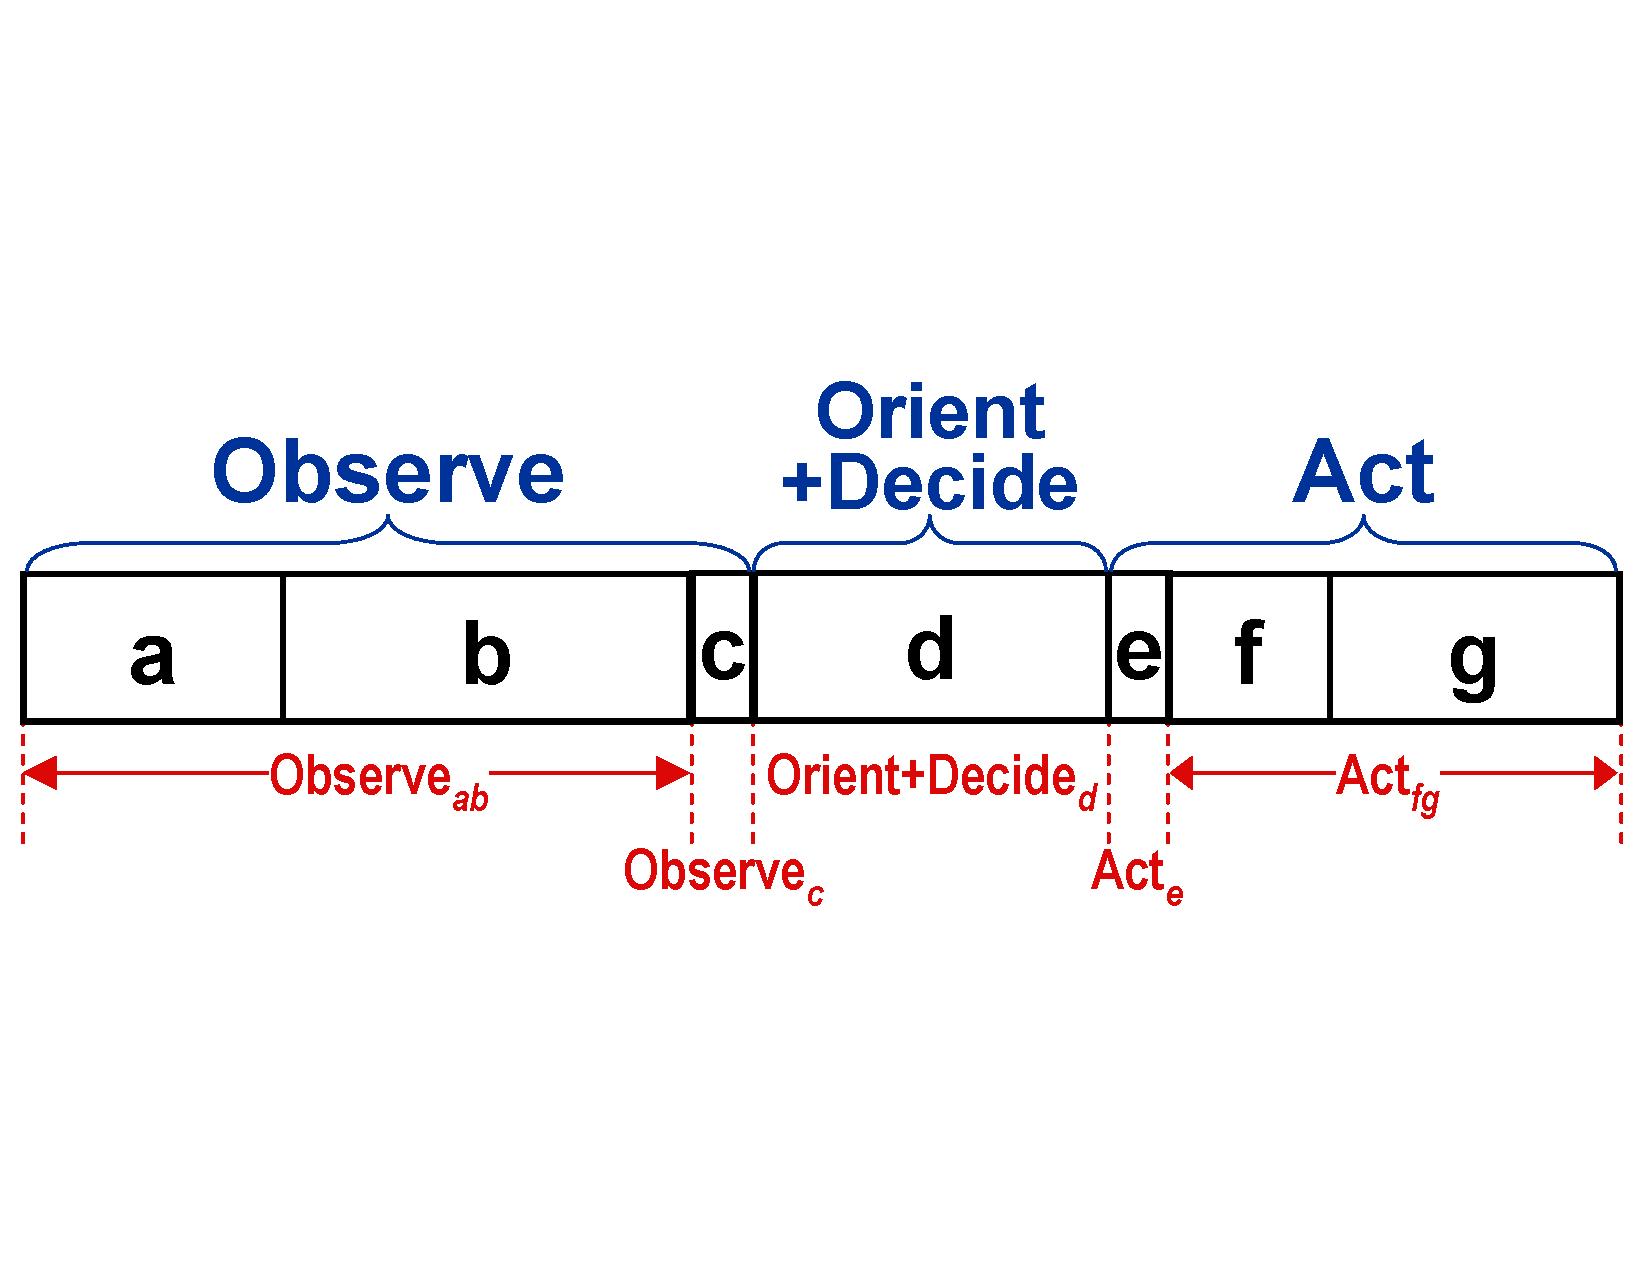
\includegraphics[width = .5\textwidth]{figs/fig-ooda-nomenclature.pdf}}
\caption{Measurable Components of the OODA Loop}
\label{fig:ooda-nomenclature}
\end{figure}

We are limited in our ability to individually measure the contribution of
components of the OODA loop. The drone sensing and pre-processing, components
(a) and (b), for instance, cannot be measured individually because the drone is
a COTS product that runs closed source software which does not allow the
ability to insert software instrumentation. Similarly, drone post-processing
and actuation must be measured together.  \Cref{fig:ooda-nomenclature} shows
the parts of the pipeline that can be measured in red.

\section{Measuring the performance of the SteelEagle pipeline}
\label{sec:steeleagle-performance-measurement}

Calculating drone-to-cloudlet latency is challenging since SteelEagle uses COTS
drones that restrict modification of its onboard software. The inability to add
software instrumentation on the drone makes it difficult to determine when a
given frame was transmitted from the drone. To circumvent this restriction,
Bala et al adapted the technique George et al used for measuring
motion-to-photon latency in augmented reality \cite{george20}.


\begin{figure}[htbp]
\centerline{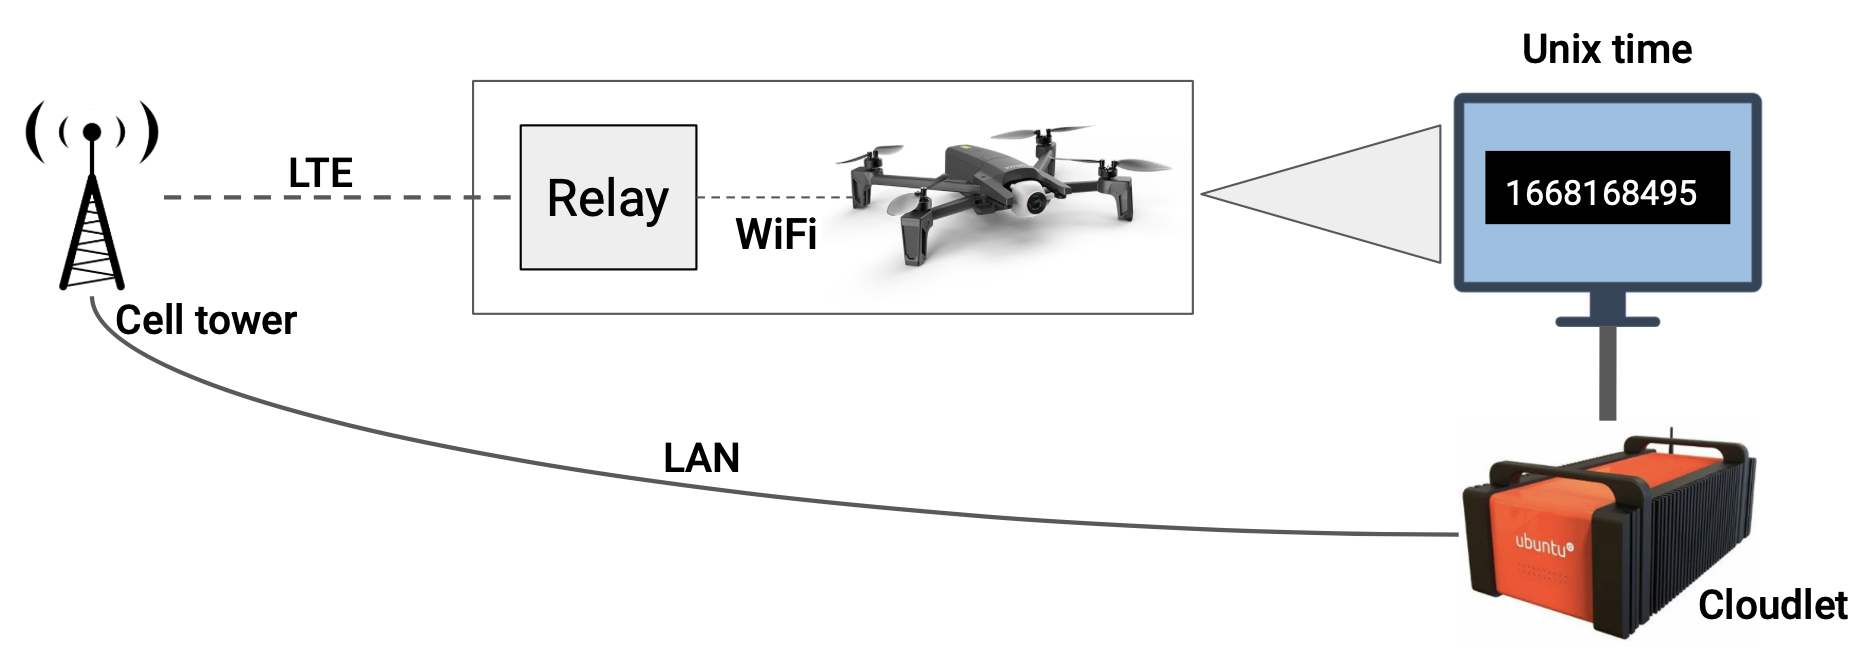
\includegraphics[width = .8\textwidth]{figs/mtp_pipeline.png}}
\caption{Technique for measuring end-to-end latency}
\label{fig:latency-measuring-technique}
\end{figure}
As shown in \cref{fig:latency-measuring-technique}, the drone is kept
stationary in a lab setting with its camera pointed at a display connected to
the cloudlet showing the current Unix timestamp at millisecond granularity. The
drone captures images containing the timestamp displayed and transmits them to
the cloudlet through the SteelEagle pipeline. The cloudlet records the
timestamp at which it receives each frame, storing the frame along with this
timestamp. To obtain the drone-to-cloudlet latency, these saved frames are
post-processed to compute the difference between the timestamps shown in each
frame and the timestamps at which they were received at the cloudlet.

\section{Experiment 1: Optimizing SteelEagle Latency}
\label{sec:exp1}

\begin{figure}[htbp]
\centerline{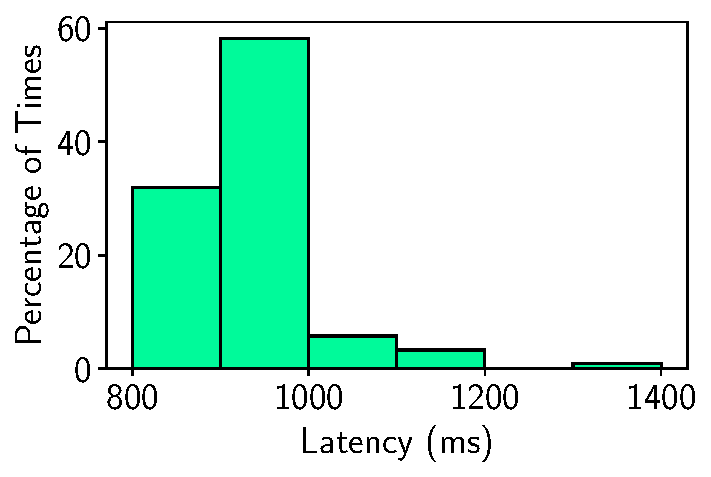
\includegraphics[width = .4\textwidth]{figs/bala_latency.pdf}}
\caption{Original SteelEagle Latency \cite{bala2024}}
\label{fig:steeleagle-original-latency}
\end{figure}

\begin{figure}[b]
    \centering
    \begin{subfigure}[t]{0.45\textwidth}
        \centering
        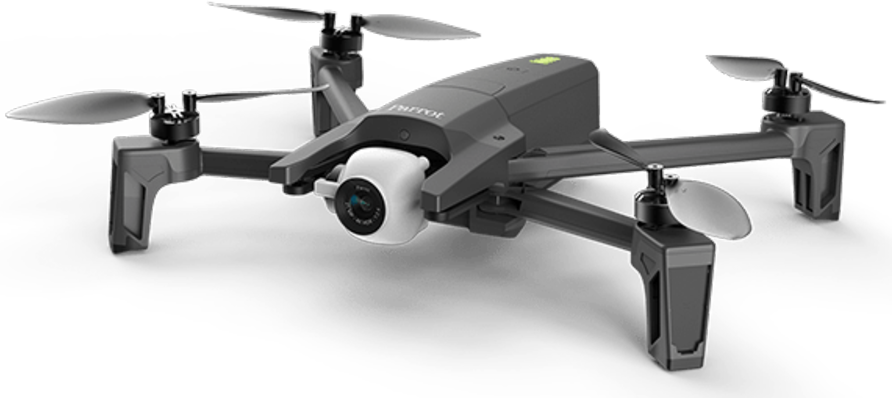
\includegraphics[height=1in]{figs/parrot-anafi.pdf}
        \caption{Parrot Anafi}
        \label{fig:parrot-anafi}
    \end{subfigure}
    \begin{subfigure}[t]{0.45\textwidth}
        \centering
        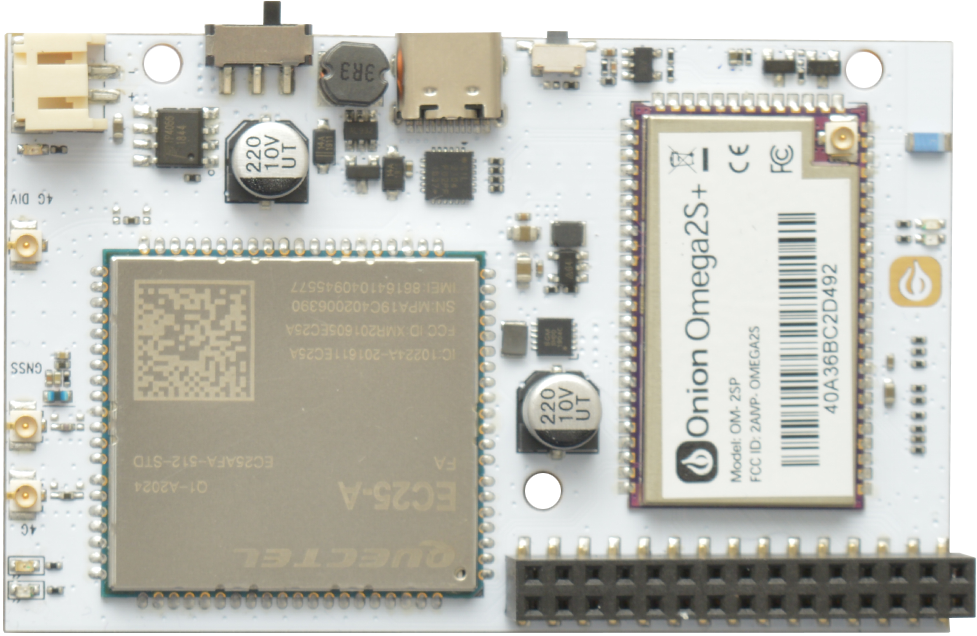
\includegraphics[height=1in]{figs/onion-omega.png}
        \caption{Onion Omega}
        \label{fig:onion-omega}
    \end{subfigure}
    \caption{The commerical-off-the-shelf components used in the SteelEagle system}
\end{figure}

The starting point of our investigation into the performance of the SteelEagle
system is the mean drone-to-cloudlet latency of 933 ms reported by Bala et al
in their benchmarking of the SteelEagle system
(\cref{fig:steeleagle-original-latency}). This includes the \observeab,
\observec, and {\orientdecide} components of the OODA pipeline.  The latency was
obtained using the Parrot Anafi drone (\cref{fig:parrot-anafi}), which
transmits a 720p H.264 RTSP stream at 30 FPS over UDP from its monocular
camera.  The Anafi uses a slice encoding and intra-refresh scheme that
disperses keyframe slices across multiple network packets
\cite{anafi_white_paper}. To reduce network bandwidth requirements, it
generates an H.264 compressed video stream using onboard hardware from the raw
frames that it obtains from its camera. Consequently, decoding of this H.264
stream is required to obtain individual video frames.  The setup uses the Onion
Omega 2 LTE (\cref{fig:onion-omega}) as a network gateway to allow the Anafi to
reach the cloudlet over LTE, since the Parrot Anafi lacks cellular
connectivity.

The described technique to measure latency does not provide a granular breakup
of the drone-to-cloudlet latency. As a result, it is not clear from the
measurements where the bottleneck resides. As an initial approach, we measure
the impact on latency when the cloudlet location and the video decoding library
used are modified. If the latency is significantly reduced by changing a
factor, we can conclude that the bottleneck resides in the corresponding
component.

\subsection{Pipeline Experimentation Parameters}

Our first experiments measure the impact on latency when the location of the
backend and the video decoding library used is changed. \Cref{tab:experiment-parameters}
summarizes the different parameters tested along these dimensions.
\begin{table}[htbp]
    \centering
    \caption{Latency Pipeline Experimentation Parameters}
    \label{tab:experiment-parameters}
    \begin{tabular}{@{}ll@{}}
        \toprule
        \textbf{Dimension} & \textbf{Parameters} \\ \midrule
        Backend Location & Cloudlet, AWS Small, AWS Big \\
        Video Decoding Library & FFmpeg, PDrAW \\ \bottomrule
    \end{tabular}
\end{table}

We now describe the details of these parameters:

\begin{itemize}

    \item \textbf{Location of backend.} Three backend locations with different
specifications, each offering varying levels of performance, are considered to
evaluate how hardware scale-up affects system latency. The SteelEagle backend
is either set up on a bare-metal server on CMU's campus, labeled ``Cloudlet'',
or on an EC2 VM in AWS East (Virginia). Two types of EC2 instances are used,
``AWS Small'' and ``AWS Big''. The CMU Cloudlet has two
Intel\textsuperscript{\textregistered} Xeon\textsuperscript{\textregistered}
E5-2699 v3 CPUs clocked at 2.30 GHz for a total of 72 vCPUs, 128GB main memory,
and an NVIDIA\textsuperscript{\textregistered}
GeForce\textsuperscript{\textregistered} GTX 1080 Ti GPU. AWS denotes a
\texttt{g4dn.xlarge} EC2 instance which has 4 vCPUs, 16GB of memory, and an
NVIDIA T4 GPU. AWS Big is a \texttt{g4dn.16xlarge} EC2 instance which has 64
vCPUs, 256GB main memory, and also an NVIDIA T4 GPU. \Cref{tab:backend-specs}
summarizes these specifications.

\begin{table}[h]
    \centering
    \caption{Specifications of Backends Used in Experiment}
    \label{tab:backend-specs}
    \begin{tabular}{@{}llll@{}}
        \toprule
        \textbf{Backend} & \textbf{vCPUs} & \textbf{Memory} & \textbf{GPU} \\ \midrule
        AWS Small & 4 & 16 GB & NVIDIA\textsuperscript{\textregistered} T4\\
        AWS Big & 64 & 256 GB & NVIDIA\textsuperscript{\textregistered} T4\\
        Cloudlet & 72 & 128 GB & NVIDIA\textsuperscript{\textregistered} GeForce\textsuperscript{\textregistered} GTX 1080 Ti\\
        \bottomrule
    \end{tabular}
\end{table}

\item \textbf{Video decoding library.} Two video decoding libraries are considered:
FFmpeg and PDrAW (pronounced ``pedro''). FFmpeg \cite{ffmpeg} is an open-source
project that offers libraries for video encoding/decoding and
multiplexing/demultiplexing. FFmpeg is known for forming a core part of the VLC
media player. We interact with FFmpeg through OpenCV~\cite{opencv}, which
offers the ability to use FFmpeg as a backend for its video capture APIs.
PDrAW \cite{pdraw} is a part of Parrot's Ground SDK software. Similar to
FFmpeg, it includes multiplexing/demultiplexing abilities and can read from the
RTSP stream generated by the Parrot Anafi drone. Unlike FFmpeg, however, PDrAW
is intended as a video player for RTSP and MP4 videos and lacks general-purpose
encoding and decoding abilities.

\end{itemize}
\subsection{Experimental Results}

\Cref{tab:latency_summary} summarizes the results obtained. For each backend
location, the latency is measured using the two different video decoding
libraries. The mean latency of 933 ms obtained by Bala et al mentioned before
used FFmpeg with the ``Cloudlet'' backend. We measured a lower mean of 888 ms
using these parameters because our experiments do not include inference time on
the cloudlet. Inference time can vary across different machine learning models,
depending on the kind of pre-preprocessing performed and architectural details
such as the number of hidden layers used.  Not including inference time, then,
allows us to focus on the contribution of other components.

\begin{table}[t]
    \centering
    \caption{Drone-to-Cloudlet SteelEagle Latency (in ms)}
    \label{tab:latency_summary}
        \sisetup{
        detect-all,
        table-number-alignment = center,
        input-decimal-markers = {.},
        group-separator={,},
        group-minimum-digits=4
    }
    \begin{tabularx}{0.6\linewidth}{@{}
        X
        c%S[table-format=3.0]
        S[table-format=3.0]
        S[table-format=3.0]
        S[table-format=3.0]
        S[table-format=4.0]@{}
    }
    \toprule
    \textbf{Configuration} & \textbf{Average} & \textbf{Median} & \textbf{p95} & \textbf{Min} & \textbf{Max} \\
    \midrule
    \multicolumn{6}{@{}l}{\textbf{Cloudlet}} \\
    FFmpeg & 888 {\small $\pm$ 30} & 887 & 917 & 838 & 1030 \\
    PDrAW   & 380 {\small $\pm$ 15} & 379 & 402 & 344 & 420 \\
    %WiFi + FFmpeg & 841.52 & 841 & 868.3 & 16.79 & 807 & 879 \\
    %WiFi + PDrAW & 340.82 & 338.5 & 373.5 & 21.82 & 298 & 419 \\
    \midrule
    \multicolumn{6}{@{}l}{\textbf{AWS Small}} \\
    FFmpeg & 536 {\small $\pm$ 75} & 521 & 600 & 473 & 936 \\
    PDrAW   & 429 {\small $\pm$ 21} & 427 & 467 & 387 & 475 \\
    \midrule
    \multicolumn{6}{@{}l}{\textbf{AWS Big}} \\
    FFmpeg & 870 {\small $\pm$ 20} & 868 & 900 & 837 & 925 \\
    PDrAW   & 367 {\small $\pm$ 20} & 365 & 392 & 327 & 416 \\
    \bottomrule
    \end{tabularx}\\
    \vspace{0.1in}
    \footnotesize
    50 samples obtained for each configuration.
\end{table}

When using FFmpeg, moving the backend from the Cloudlet to AWS Small leads to
an extreme drop in latency, with a reduction in p95 latency from 917 ms to 600
ms (\Cref{tab:latency_summary}). This amounts to a 1.5$\times$ speedup,
with an improvement of over 300 ms. \Cref{fig:box_plots} shows an interesting
trend. The latency for AWS Small, which has the weakest computation power, is
the lowest when using FFmpeg and the highest when using PDrAW.  This
discrepancy is unexpected, as we anticipate AWS Small to perform consistently
across both setups.

This led to the hypothesis that FFmpeg's performance degrades with increased
parallelism, as it struggles to scale effectively with higher CPU counts.  To
test this hypothesis, measurements were obtained by varying the number of
threads used for FFmpeg from one to six (see \Cref{fig:threads_box_plot}).  The
OpenCV option \texttt{CAP\_\allowbreak PROP\_\allowbreak N\_\allowbreak
THREADS} was used to set the number of threads used for the FFmpeg backend.
The results show that the latency increases as we increase the number of threads,
suggesting that FFmpeg suffers from negative-scale out attributes. Adding more
threads to FFmpeg hurts latency.

\begin{figure}[htbp]
\centerline{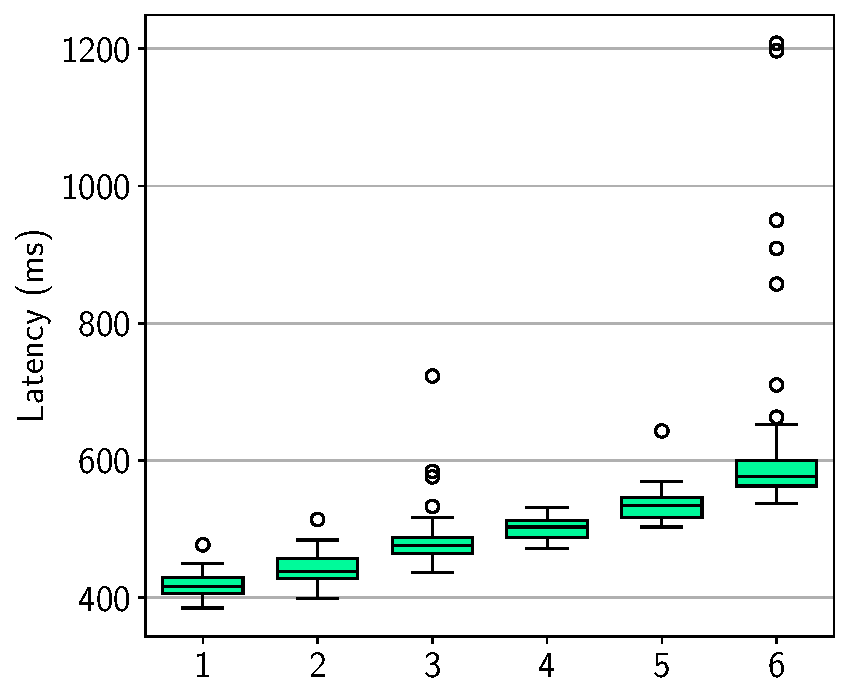
\includegraphics[width = .4\textwidth]{figs/threads_box_plot.pdf}}
\caption{Latency vs. Number of FFmpeg Threads}
\label{fig:threads_box_plot}
\end{figure}

\begin{figure}[htbp]
    \centering
    \begin{subfigure}[t]{0.45\textwidth}
        \centering
        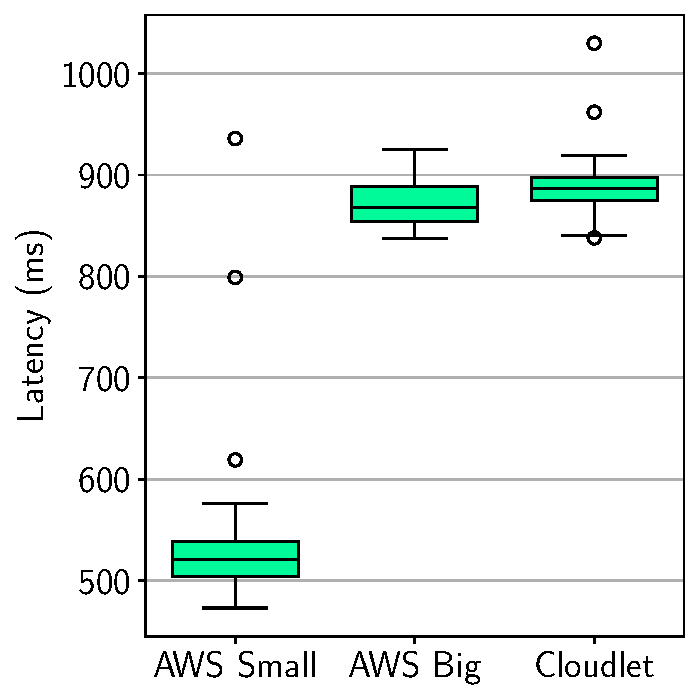
\includegraphics[height=2.5in]{figs/ffmpeg_box_plot.pdf}
        \caption{FFmpeg}
        \label{fig:ffmpeg_box_plot}
    \end{subfigure}
    \begin{subfigure}[t]{0.45\textwidth}
        \centering
        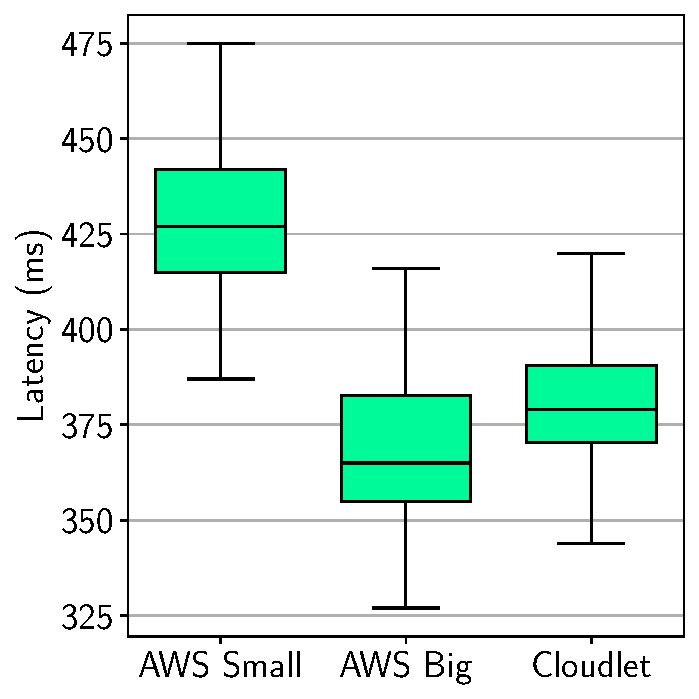
\includegraphics[height=2.5in]{figs/pdraw_box_plot.pdf}
        \caption{PDrAW}
        \label{fig:pdraw_box_plot}
    \end{subfigure}\vspace{1mm}\\
        \footnotesize{Each box extends from the first quartile ($Q_1$) to the third quartile ($Q_3$), with a line at the median. Whiskers extend from the box to the farthest data point lying within 1.5x the inter-quartile range ($IQR = Q_3-Q_1$) from the box. Circles represent outliers. 50 samples obtained for each configuration.}
    \caption{Latency Across Backend Locations Using Different Video Decoding Libraries}
    \label{fig:box_plots}
\end{figure}

Across all backend locations, we achieve the lowest latency by replacing FFmpeg
with PDrAW for video decoding.  For CMU Cloudlet, latency reduced
from 917 ms to 402 ms by switching to PDrAW, a speedup of almost 2.3$\times$.

\begin{figure}[htbp]
\centerline{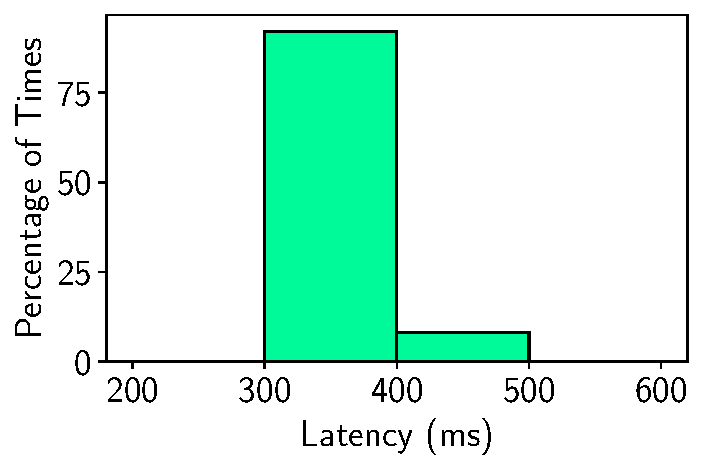
\includegraphics[width = .4\textwidth]{figs/pdraw_latency.pdf}}
\caption{Optimized SteelEagle Latency using PDrAW for Video Decoding}
\label{fig:steeleagle_optimized_latency}
\end{figure}

\section{Experiment 2: A More Structured Benchmarking Approach}
\label{sec:exp2}
